\begin{blocksection}
\question What would Python display? If an error occurs, write "Error". If a function is displayed, write "Function". If nothing is returned, write "Nothing".

\begin{lstlisting}
>>> a = [1, 2]
>>> b = a
>>> print(a.append([3, 4]))
\end{lstlisting}
\begin{solution}[0.25in]
\begin{lstlisting}
None
\end{lstlisting}
\end{solution}

\begin{lstlisting}
>>> a
\end{lstlisting}
\begin{solution}[0.25in]
\begin{lstlisting}
[1, 2, [3, 4]]
\end{lstlisting}
\end{solution}

\begin{lstlisting}
>>> b
\end{lstlisting}
\begin{solution}[0.25in]
\begin{lstlisting}
[1, 2, [3, 4]]
\end{lstlisting}
\end{solution}

\begin{lstlisting}
>>> c = a[:]
>>> a[0] = 5
>>> a[2][0] = 6
>>> c
\end{lstlisting}
\begin{solution}[0.25in]
\begin{lstlisting}
[1, 2, [6, 4]]
\end{lstlisting}
\end{solution}

\begin{lstlisting}
>>> a.extend([7, 8])
>>> a += [9]
>>> a += 10
\end{lstlisting}
\begin{solution}[0.25in]
\begin{lstlisting}
TypeError: 'int' object is not iterable
\end{lstlisting}
\end{solution}

\begin{lstlisting}
>>> a
\end{lstlisting}
\begin{solution}[0.25in]
\begin{lstlisting}
[5, 2, [6, 4], 7, 8, 9]
\end{lstlisting}
\end{solution}
\end{blocksection}
\begin{blocksection}
\begin{lstlisting}
>>> print(c.pop(), c)
\end{lstlisting}
\begin{solution}[0.25in]
\begin{lstlisting}
[6, 4] [1, 2]
\end{lstlisting}
\end{solution}
\end{blocksection}

\begin{blocksection}
\begin{guide}
\begin{itemize}
	\item Draw a box and pointer diagram or utilize \url {https://tinyurl.com/1at3617r}
	\item Mention shallow vs. deep copying. In general, most operators involving python lists perform shallow copying: i.e. slicing, list(...), etc.
	\item If you have enough time, it is helpful for students to make a chart which the different operators and identify when to mutate or create a new list.
    \item Do remind students of the difference between \lstinline{a += b} and \lstinline{a = a+b}. The former is essentially \lstinline{a.extend(b)}, while the latter creates a new list consisting of all the elements of \lstinline{a} and \lstinline{b} combined and binds it to \lstinline{a}.
\end{itemize}
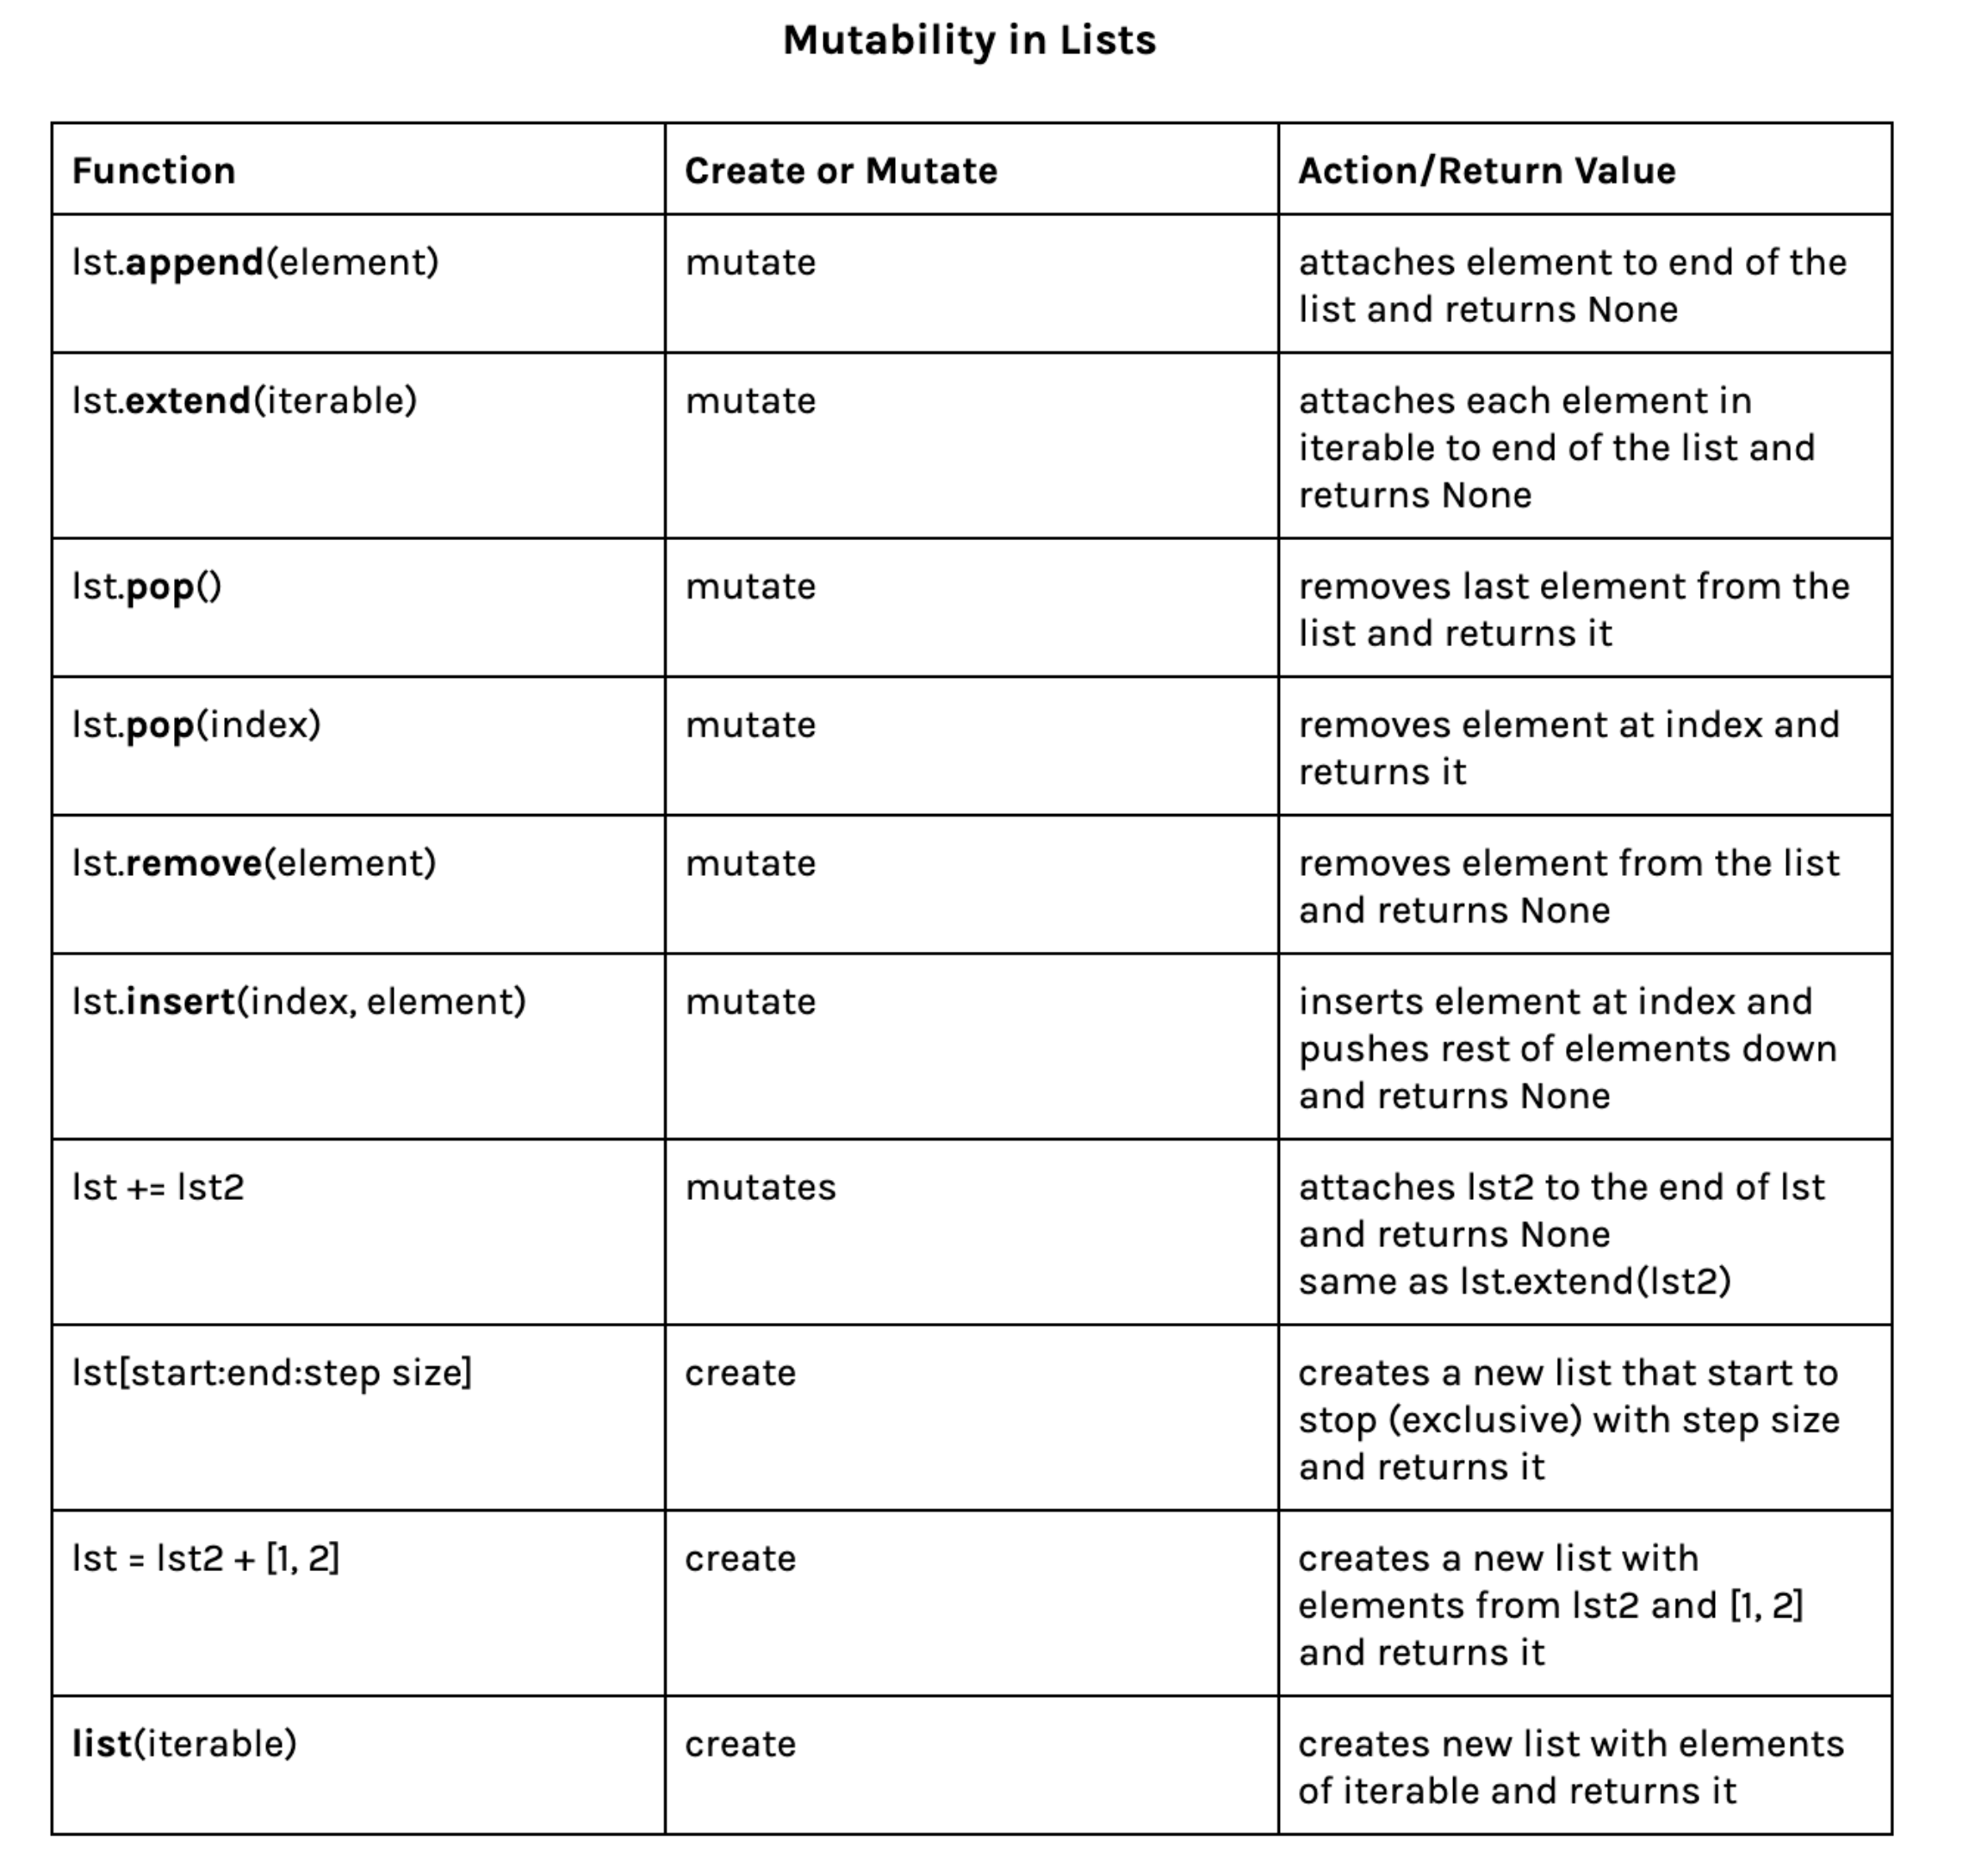
\includegraphics[width=.9\textwidth]{list-mutation.png}
\text{(credits: Mihira Patel)}
\end{guide}
\end{blocksection}
